\section{Aufbau}
\label{sec:Aufbau}


\begin{figure}[H]
 \centering
 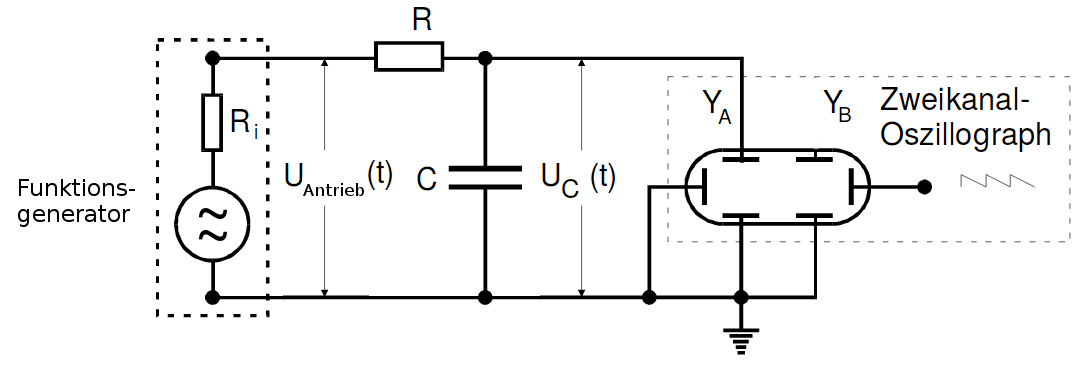
\includegraphics[width=\linewidth-100pt,height=\textheight-100pt,keepaspectratio]{content/aufbau353.png}
 \caption{Messchaltung zur Bestimmung der Zeitkonstante $\tau$ \cite{V353}.}
 \label{fig:Aufbaua}
\end{figure}
Die obige Schaltskizze zeigt einen Versuchsaufbau zur Messung der spezifischen
 Zeitkonstante $\tau$ eines $RC$-Kreises. Im Kern besteht dieser aus einem $RC$-Glied, welches über einen
  Funktionsgenerator einer periodischen Spannung unterliegt. Um den
   Spannungsverlauf am Kondensator zu untersuchen wird zudem ein
    Zweikanaloszilloskop am Kondensator zugeschaltet. Zunächst wird nur ein Kanal verwendet.
